\section{Existing Services}

The tourism industry exists since, at least, the 19th century,
but it was impacted by some significant chapters of human technology, which lead to an increased and sustained growth of the market size. First, during the 1920's, the development of commercial aviation meant a significant impact on the industry, shifting the transportation focus to the airplane. Much later, during the 90's, the establishment of the internet led to some changes in the market because airlines were able to sell directly to the passengers \cite{tourism_tec}. More recently, the widespread use of mobile phones lead to a new increase in the markets size. In 2016, the direct contribution of the tourism industry for the GDP was over 2.3 trillion dollars, while the total contribution was over 7.6 trillion dollars\cite{travel_report}.

The market size growth of the tourism industry is sustained by traveling agencies, whose main function is to serve as an agent,  advertising and selling products and services on behalf of other \cite{book_tourism}. These services usually include, but are not limited to, transportation, accommodation, insurance, tours and other tourism associated products. The focus of this section will be given to the overview of the search tools provided by online travel agencies upon requesting information regarding a single-flight, as well as round and multi-city trips.   

Online Traveling Agencies are websites and applications which offer traveling services or reviews, as illustrated in figure \ref{fig:ota_services}. Most OTA function as a metasearch engine, which means that they search multiple independent travel services providers. Furthermore, this is the main differentiator from the search engines provided by OTA's, and those from direct travel suppliers, as are the websites of individual airlines. Direct travel suppliers are limited to display the results of their own services. On the other hand, OTA usually do not own any travel services but serve solely as an intermediary between traveler and travel services provider. In some cases, these metasearch engines may resort to web scraping in order to get real-time data on the flights provided by different airlines. Recent reports show that while OTA are increasing its market share, direct travel suppliers still account for 57\% of the total online travel consumption \cite{OTA_industry_report}.


\begin{figure}[]
  \centering
  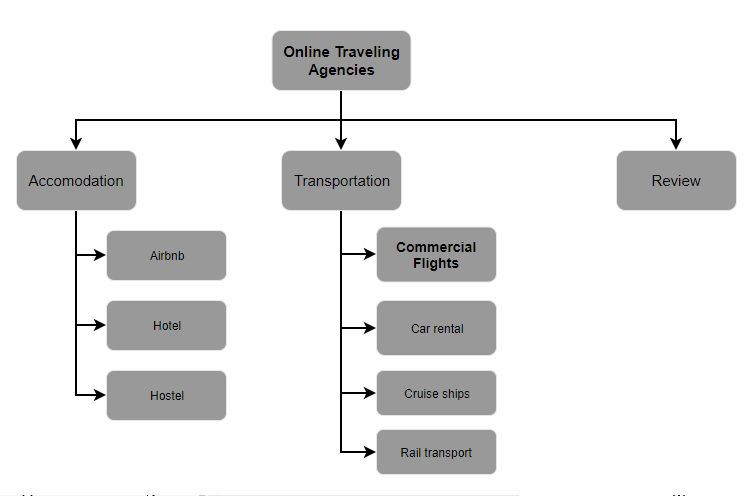
\includegraphics[width=\textwidth]{./Figures/introduction/services_OTA.png}
  \caption{The different services provided by Online Traveling Agencies}
  \label{fig:ota_services}  
\end{figure}

In order to better understand the difference between OTA's and direct travel suppliers, 
consider the case of a user searching for a simple round flight between two cities. 
If this user visits an individual airline website, the flight results presented are limited to those offered by this airline.
However, there is no guarantee that the airline flies the user defined route.
Furthermore, even if there is such a route, it is possible that this route is not flown every day.
Note that these two types of problems are very common, especially in low-cost airlines.
In contrast, the same round flight search on a metasearch engine of some OTA 
will produce a variety of results which include several different airlines.
Finally, since OTA aggregate data from different airlines and other meta searches,
it is less likely for the two problems described above to occur using the OTA search tools.
In conclusion, collecting data from multiple sources usually results in a higher variety and quality of results.

Despite the variety of services provided by OTA, this section will focus only on making a review of the existing search tools available for the commercial flight
transportation segment. This analysis will be made from both the user and the developer point of view
because the offered services often vary according to this. 


\subsection{User Search Tools}
Depending on the specific application, online traveling agencies may offer services which
include transportation and accommodation. The focus of this section is to create an extensive
overview of the search tools available for finding commercial flights. 
In order to classify the search tools, the results will be grouped 
according to the \textit{trip type}:

\begin{itemize}
  \item single/round flight;
  \item multi-city trip;
\end{itemize}

This overview will also focus on the different search utilities provided 
by the search applications. Thus, it will analyze the ability to:

\begin{itemize}
  \item search over a range of start dates - \textbf{DR};
  \item present a price overview as a function of time - \textbf{PO};
  \item present different results for different criteria - \textbf{VR};
  \item display an interactive map - \textbf{Map};
\end{itemize}

There are other search utilities, presented by some online search applications,
which will not be subject of study. These include:

\begin{itemize}
  \item price monitoring and alerting service;
  \item analysis of the probability of price fluctuations;
  \item information about alternative flights;
  \item automatic caching for future usage;
\end{itemize}

This analysis will be considered for the major flight search applications,
which include, for example, Google Flights, Momondo, Skyscanner, Kayak, and Kiwi.



\subsubsection*{Single/Round flights}


In order to evaluate the search utilities provided by every flight search application,
as well as the actual price displayed, the same search will be performed over 
all applications. In particular, this search was executed over a month before the 
actual start date, and corresponds to:

\begin{itemize}
\item \textbf{S} - single flight - from Lisbon, to Amsterdam, at 8/6/2018;
\item \textbf{R} - round flight - from Lisbon, to Amsterdam, at 8/6/2018, for a duration of 3 days;
\end{itemize}

Table \ref{tab:simple_flights_analysis} displays 
the results of the search performed over the different applications,
together with a checklist specifying which search utilities are provided.
It is also worth noting that the price displayed in this table might not correspond to
the actual final price. For example, Edreams is well known for charging extra fees only upon the ticket purchase. 

\begin{table}[h]
  \centering
  \caption{Comparison of the search results, and search utilities, of different online flight search applications, for single and round flights.}
  \label{tab:simple_flights_analysis}
  \begin{tabular}{|l|l|l|l|l|l|l|}
  \hline
  company             & DR                & PO         & VR         & Map        & S                          & R                           \\ \hline
  Google Flights      & $\checkmark$              & $\checkmark$ &            & $\checkmark$ & 65                         & 127                         \\ \hline
  Expedia             &                              &            &            &            & 81                         & 167                         \\ \hline
  Booking.com / Kayak &                              &            & $\checkmark$ & $\checkmark$ & 67                         & 126                         \\ \hline
  Momondo             &                              & $\checkmark$ & $\checkmark$ &            & 62                         & \cellcolor[HTML]{C0C0C0}102 \\ \hline
  TripAdvisor         &                              &            &            &            & \cellcolor[HTML]{C0C0C0}56 & 124                         \\ \hline
  cheapflights.com    &                              &            &            &            & 75                         & 150                         \\ \hline
  Adioso              & $\checkmark$        &            & $\checkmark$ &            & 69                         & 137                         \\ \hline
  kiwi                & $\checkmark$        & $\checkmark$ & $\checkmark$ & $\checkmark$ & 76                         & 224                         \\ \hline
  SkyScanner          & $\checkmark$              & $\checkmark$ &            &            & 65                         & 127                         \\ \hline
  Edreams             & $\checkmark$              &            & $\checkmark$ &            & \cellcolor[HTML]{C0C0C0}56 & 116                         \\ \hline
  \end{tabular}
\end{table}

From the analysis of table \ref{tab:simple_flights_analysis}, it is possible to conclude that, for single and round flights:

\begin{itemize}
  \item different applications provide significantly different results. Single and round flight prices vary up to 44\% and 120\% respectively;
  \item half of the applications do not provide date range support;
  \item half of the applications do not provide price overview as a function of time;
  \item most applications do not present an interactive map;
\end{itemize}




\subsubsection*{Multi-city trips}


Following the same methodology as in the previous section, the same multi-city trip search will be performed 
on the different applications, and the result is presented as \textbf{M} in table \ref{tab:multi_city_analysis}. This search corresponds to:

\begin{itemize}
  \item single flight from Lisbon to Amsterdam, at 8/6/2018, for a duration of 3 days;
  \item single flight from Amsterdam to Berlin, at 11/6/2018, for a duration of 3 days;
  \item single flight from Berlin to Lisbon, at 14/6/2018;
\end{itemize}

It is worth noting that all flight search applications which currently perform multi-city trips,
do it in the exact same way: a multi-city trip corresponds to a collection of single flights,
which must specify the origin and destination, together with a single start date.

This case corresponds to a very inefficient search for a variety of reasons.
First of all, it constrains the search to one particular route. Second, it does not allow 
any kind of flexibility around the start date or duration of stay associated to each city. 
And finally, changing one parameter of the search might affect the rest of the trip.

Once again, the results of the search, together with the search utilities, are presented in table \ref{tab:multi_city_analysis}.
Note that MTCS stands for the ability to search for multi-city trips, as those specified above.

\begin{table}[h]
  \centering
  \caption{Comparison of the search results, and search utilities, of different online flight search applications, for multi-city trips.}
  \label{tab:multi_city_analysis}
  \begin{tabular}{|l|l|l|l|l|l|l|}
  \hline
  company             & MTCS       & DR  & PO         & VR         & Map                      & M                           \\ \hline
  Google Flights      & $\checkmark$ &       &            &            &                          & 184 \\ \hline
  Expedia             & $\checkmark$ &        &            &            &                          & 420                         \\ \hline
  Booking.com / Kayak & $\checkmark$ &        &            &            &                          & 191                         \\ \hline
  Momondo             & $\checkmark$ &        &            & $\checkmark$ &                          & \cellcolor[HTML]{C0C0C0}178 \\ \hline
  TripAdvisor         & $\checkmark$ &        &            & $\checkmark$ &  & 238                         \\ \hline
  cheapflights.com    &            &        &            &            &                          &                             \\ \hline
  Adioso              &            &        &            &            &                          &                             \\ \hline
  Kiwi                & $\checkmark$ &        & $\checkmark$ &            &                          & 226                         \\ \hline
  SkyScanner          & $\checkmark$ &        &            & $\checkmark$ &                          & 238                         \\ \hline
  Edreams             & $\checkmark$ &        &            &            &  & 333                         \\ \hline
  \end{tabular}
\end{table}

From the analysis of table \ref{tab:simple_flights_analysis}, it is possible to conclude that, for multi-city trips:

\begin{itemize}
  \item different applications provide significantly different results, which vary up to 135\%;
  \item most applications provide (limited) multi-city trip search; 
  \item most applications do not present different results for different search criteria;
  \item no application offers the ability to perform multi-city trips on a range of start dates; 
  \item no applications displays an interactive map;
\end{itemize}
% Depending on the specific application,
% online traveling agencies may offer services which include 
% transportation and accomodation. The focus of this section 
% is to create an extensive overview of the search tools available 
% for finding commercial flights.

% The websites associated to commercial flight metasearch engines include,
% but are not limited to, Google Flights, Booking.com, Tripadvisor,
% cheapflights.com, Momondo, Expedia, Edreams, Kayak, Kiwi and Skyscanner. 

% The search functions provided by these websites can 
% be grouped according to trip size: single, round and multi city trip.
% They can also be grouped according to their ability to 
% search for flights starting on a particular date or range of dates.
% There are some applications which also focus on presenting different relevant results,
% organizing their results by price, duration and a mix of both.
% Some of these websites also include an interactive map,
% which displays the flights prices, and allows user to 
% create and visualize the selected routes.

% In order to create an extensive collection of the available search tools  in each website,
% the same two queries were performed. The first, a single flight from Lisbon to Amsterdam
% at 8/6/2018. The second, a round flight involving these two cities and start date,
% and a duration of stay of 3 days. The table below presents the price results 
% of this search, aswell as the search tool options available upon search.

% \begin{table}[]
%   \centering
%   \caption{Search results across several applications. Search tools provided according to application}
%   \label{my-label}
%   \begin{tabular}{|l|l|l|l|l|l|l|l|}
%   \hline
%                       & RD               & VD         & PO         & VR         & Map        & A                          & B                           \\ \hline
%   Google Flights      & $\checkmark$ $\star$ &            & $\checkmark$ &            & $\checkmark$ & 65                         & 127                         \\ \hline
%   Expedia             &                  &            &            &            &            & 81                         & 167                         \\ \hline
%   Booking.com / Kayak &                  &            &            & $\checkmark$ & $\checkmark$ & 67                         & 126                         \\ \hline
%   Momondo             &                  &            & $\checkmark$ & $\checkmark$ &            & 62                         & \cellcolor[HTML]{C0C0C0}102 \\ \hline
%   TripAdvisor         &                  &            &            &            &            & \cellcolor[HTML]{C0C0C0}56 & 124                         \\ \hline
%   cheapflights.com    &                  &            &            &            &            & 75                         & 150                         \\ \hline
%   Adioso              & $\checkmark$       & $\checkmark$ &            & $\checkmark$ &            & 69                         & 137                         \\ \hline
%   kiwi                & $\checkmark$       & $\checkmark$ & $\checkmark$ & $\checkmark$ & $\checkmark$ & 76                         & 224                         \\ \hline
%   SkyScanner          & $\checkmark$ $\star$ &            & $\checkmark$ &            &            & 65                         & 127                         \\ \hline
%   Edreams             & $\checkmark$ $\star$ &            &            & $\checkmark$ &            & \cellcolor[HTML]{C0C0C0}56 & 116                         \\ \hline
%   \end{tabular}
%   \end{table}

% Other services included by some of these websites are:
% \begin{itemize}
%   \item price tracking
%   \item probability of price variations in the following dates 
%   \item alternative flight information 
%   \item automatic caching for further usage 
% \end{itemize}

 
% \begin{table}[]
%   \centering
%   \caption{Multicity search results and tools.}
%   \label{my-label}
%   \begin{tabular}{|l|l|l|l|l|l|l|l|}
%   \hline
%                       & MTCS       & RD & VD & PO         & VR         & Map                      & C                           \\ \hline
%   Google Flights      & $\checkmark$ &    &    &            &            &                          & \cellcolor[HTML]{C0C0C0}184 \\ \hline
%   Expedia             & $\checkmark$ &    &    &            &            &                          & 420                         \\ \hline
%   Booking.com / Kayak & $\checkmark$ &    &    &            &            &                          & 191                         \\ \hline
%   Momondo             & $\checkmark$ &    &    &            & $\checkmark$ &                          & \cellcolor[HTML]{FFFFFF}178 \\ \hline
%   TripAdvisor         & $\checkmark$ &    &    &            & $\checkmark$ &  & 238                         \\ \hline
%   cheapflights.com    &            &    &    &            &            &                          &                             \\ \hline
%   Adioso              &            &    &    &            &            &                          &                             \\ \hline
%   Kiwi                & $\checkmark$ &    &    & $\checkmark$ &            &                          & 226                         \\ \hline
%   SkyScanner          & $\checkmark$ &    &    &            & $\checkmark$ &                          & 238                         \\ \hline
%   Edreams             & $\checkmark$ &    &    &            &            &  & 333                         \\ \hline
%   \end{tabular}
% \end{table}

% Note about multi city search.
% Every website performs multi city searches in the exact same way, which is stacking up single flights 
% to compose a multi city trip.
% This however, has a number of inconvenients. The first is that the trip route is fixed to a certain order,
% and, more impactful, to certain dates.
% The single flights which are stacked to compose a single flight are not served by broader queries,
% but are limited to a pair of cities and one start date. This leads to a second inconvinent,
% which is the inflexibility of the search. Changing the start time or the route implies changing the query of all flights.
% This produces both a slow and inextensive search.  


\subsection{Developer Search Tools}

% For a developer which intends to create a meta flight search by its own,
% there are some well estabilished online traveling which offer free, limited or paid 
% access to their own flight API. Between the list of companies which offer these services 
% are Google, Kiwi, Skyscanner, Amadeus and Expedia.

% Despite the variety of publicly available API's, there are only very few which are free and available to anyone.
% Some companies (google) limit their free search query usage, while others (skyscanner) offer there services only to enterprises. 
% Amadeus and Expedia are free Api's, but their services are focused on the USA market,
% and thus have a limited of routes.

% The best free public API found is Kiwi. The access to the API is completly free and unlimited. 
% It includes the possibility to search for cached flights, real time data, and even hotal prices.
% The usage of this API also includes complex queries, as the search of flights 
% during extended time periods, and even variable duration. 
% Finally, there is also the possibility to search for multiple, well defined, flights at once, 
% by aggregating up to 9 single flight queries. 

For a developer that intends to create a flight meta-search engine, a way to access flight
data is essential. There are some online traveling agencies which extend their API for public
consultation. Amongst the services that these public API’s offer, are the possibility of searching
for cached, and sometimes, real-time flight data. In some cases, these API's extend their range of
services and include endpoints for the consultation of hotel information, car-rental, cruise ships
and even railroad data \cite{expedia_docs, skyscanner_docs}.

Usually, these type of content provider benefits from sharing their API, because it generally
increases their traffic and the number of potential clients and bookings. In most cases, metasearch
engines do not handle booking directly, but redirect to the original content provider. In
this case, the content provider retains the entirety of the booking fees. In the case where the
meta-search engine does manage the booking, the content provider retains the majority of the
booking fee’s, while the second party may retain some share of these revenues \cite{skyscanner_pricing}.

Amongst the companies which extend their API for third party are Google, Skyscanner, Expedia and Kiwi.
These API usually operate as a \textit{free}, \textit{limited} or \textit{private} service.
For example, while Expedia and Kiwi offer free publicly accessible API's,
Skyscanner has a \textit{private companies only} \cite{skyscanner_private} policy, denying any free public consultation for educational purposes.
In its turn, Google has a free, but limited API, in the sense that only 50 free daily queries are available,
and anything beyond that has an associated cost \cite{google_qpx}.

Due to the educational purpose of this work, the interest in a flight API is limited to those which are free.
Considering the different API's that were consulated and analyzed, Kiwi's free public API stroke as the most useful, efficient and fast.
The major search utilities that this API offers are \cite{kiwi_api}:
\begin{itemize}
  \item access to relevant information about cities, airport data and airline companies;
  \item access to flight information, with flexible queries;
  \item the possibility of specifying multiple start dates;
  \item the possibility of specifying a variable duration associated to a return flight;
  \item flexibility on the specification of the origin and destination;
  \item possibility to produce multi-flight queries, by grouping up to a total of 9 simple flight queries.
\end{itemize}

Note that although Kiwi, and other companies, enable the possibility of quering 
for multiple flights at once, each flight must specify a particular pair of cities and date.
Thus, this is a constrained multi-city search, and does not actually give 
any information about the best route, schedule or set of flights for a multi-city trip.  







% \subsection{Kiwi Traveling Salesman Challenge}

% Kiwi, a well estabilished online Traveling Agency, with a high value application, search engine and API, 
% issued a public online Traveling Salesman Challenge, \textbf{cite}. In this challenge, they recognize that, in some cases, 
% users do not care about the order in which the cities are visited. They also mention that there exists a huge market for this,
% but ackowledge the complexity of the problem, stating that removing the order constraint, the problem becomes NP-hard.
% The objective of this challenge was to solve time-dependent TSP instances with up to 300 cities. 
% The problem under consideration presented several simplifications relative to the real life problem,
% by considering no travel time, and a duration of 1 time unit for each city. This formulation is equal to the 
% one presented in section \ref{sec:TDTSP_ILP}.  